\section{Decay with Decay Partners at Different Distances}
\label{sec:partners}

To fully understand the spectra of clusters with several possible
initially ionized atoms with multiple decay partners it is necessary to
understand the properties of the decay of a single pair of atoms. As can be seen
from Eqs. (\ref{equation:E_sec}) -- (\ref{equation:E_fin}),
the kinetic energy of the ICD electron follows an
$1/R$-behaviour shown in Figure \ref{figure:model_RE} for the case
of a neon dimer at different distances.

\begin{figure}[h]
 \centering
 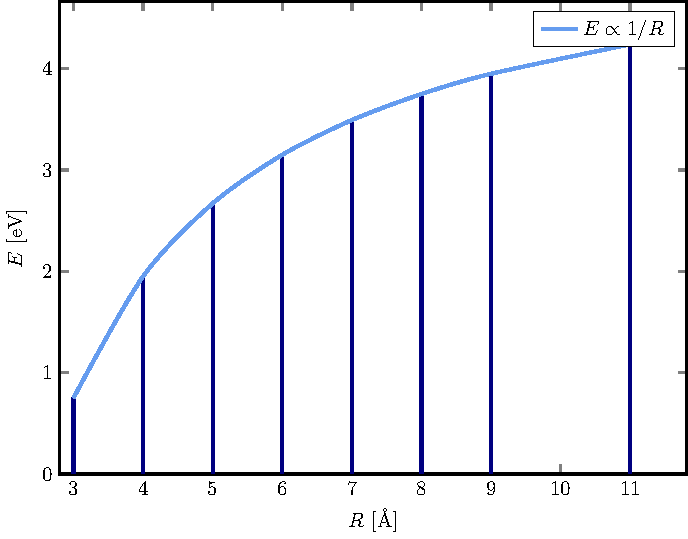
\includegraphics[width=\columnwidth]{pics/model_RE.pdf}
 \caption{Kinetic energy of the ICD electron depending on the interatomic
          distance of the two atoms involved in the decay within the
          asymptotic approximation. The kinetic energy shows a $1/R$
          behaviour and hence distance changes at small distances lead
          to larger changes in the kinetic energy than at larger distances.}
 \label{figure:model_RE}
\end{figure}
From this diagram it can already be
seen that the kinetic energies stemming from equidistant peaks of
\unit[3]{\AA}, \unit[4]{\AA}, \unit[5]{\AA}, \dots ,\unit[11]{\AA} are
not equidistant in their energy difference but rather decrease for
an increasing interatomic distance.

The corresponding decay widths $\Gamma$ depending on the interatomic
distance are shown in Figure \ref{figure:model_RGamma}. They show an
asymptotic $1/R^6$-behaviour such that the decay widths from an interatomic
distance of \unit[7]{\AA} on are too small to be seen in the
figure. This means that in case of a neon dimer with an internuclear distance
of \unit[3]{\AA}, a decay with one decay partner at twice the internuclear
distance of the neon dimer is very unlikely, but that interactions with
decay partners at shorter distances can not in general be neglected.

\begin{figure}[h]
 \centering
 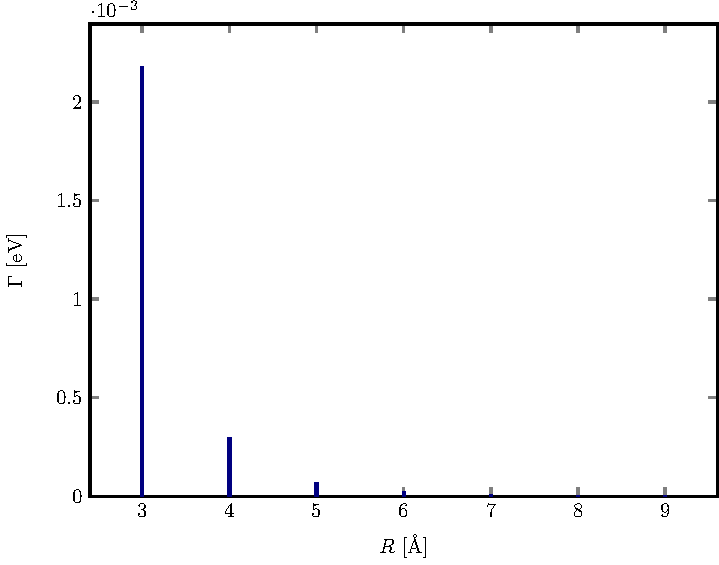
\includegraphics[width=\columnwidth]{pics/model_RGamma.pdf}
 \caption{Decay widths for different interatomic distances following an
          asymptotic $1/R^6$-behaviour. For distances larger than twice
          the shortest distance considered the peaks are not visible in this
          plot.}
 \label{figure:model_RGamma}
\end{figure}

A similar picture is given by the hypothetical ICD-electron spectrum for
decay partners at distances of \unit[3]{\AA}, \unit[4]{\AA}, \dots,
\unit[11]{\AA} shown in Figure \ref{figure:model_EGamma}. Here, the kinetic
energy of the ICD electron is depicted on the abscissae while the decay
width $\Gamma$ is plotted on the ordinate. Since the decay width is proportional
to the decay rate and hence the decay propability, these spectra can directly
be compared to experimental ICD electron spectra.

\begin{figure}[h]
 \centering
 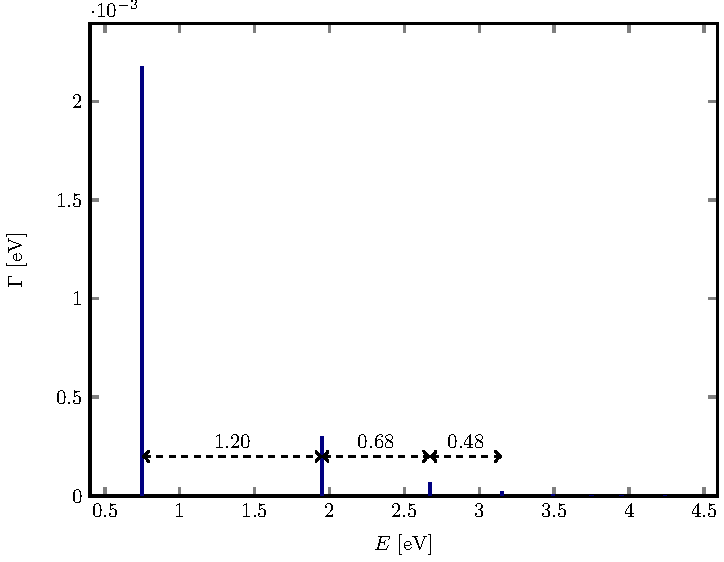
\includegraphics[width=\columnwidth]{pics/model_EGamma.pdf}
 \caption{ICD electron spectrum for interaction partner distances of
          \unit[3]{\AA}, \unit[4]{\AA}, \unit[5]{\AA}, \dots ,\unit[11]{\AA}.
          The energy difference between equidistant interaction partners
          decreases with increasing distance. For the case of Ne$_2$ pairs
          these energy differences between the peaks stemming from different
          interatomic distances are given by:
          \unit[3]{\AA},\unit[4]{\AA} $\rightarrow$ \unit[1.20]{eV},
          \unit[4]{\AA},\unit[5]{\AA} $\rightarrow$ \unit[0.68]{eV} and
          \unit[5]{\AA},\unit[6]{\AA} $\rightarrow$ \unit[0.48]{eV}.
          This means that the spectrum is better resolved for smaller distances
          and that small distance changes like vibrations will mainly affect
          this lower energy part of the spectrum.
}
 \label{figure:model_EGamma}
\end{figure}

The first and dominant peak stems from the decay with a decay
partner at a distance of \unit[3]{\AA}. The energy distance to the next peak
stemming from a decay with a decay partner with an internuclear distance of
\unit[4]{\AA} is found at a \unit[1.20]{eV} higher kinetic energy and the
energy difference to the next peak stemming from a \unit[5]{\AA} distant
decay partner is further \unit[0.68]{eV} higher. The increase of kinetic
energy of the ICD electron is caused by a decrease of Coulomb repulsion between
the interaction partners in the final state and therefore, the additional
excess in energy is converted into kinetic energy of the emitted ICD electron.
The energy difference between the peaks shown in Figure \ref{figure:model_EGamma}
decreases with an increasing distance of decay partners and at the same time
the kinetic energy
of the ICD electron. This means that for smaller interatomic distances and
comparably low kinetic energies of the ICD electron, the spectrum has a higher
resolution.
Therefore, a peak structure might be visible for the decay with nearest
neighbours (or the closest atoms with energetically allowed decay channels)
but not necessarily for all different kinds of interaction partners at larger
distances.

%\begin{figure}
% \centering
% \includegraphics[width=\textwidth]{pics/}
% \caption{}
% \label{}
%\end{figure}
